%
% Presentación para congreso.
% Proyecto Lovelace.
%

\documentclass{beamer}
\usepackage{array}
\usepackage{formato}
\newcommand{\Titulo}{\textbf{Un vistazo a la tokenización}}
\newcommand{\Fecha}{Puebla, 14 de octubre de 2018}
\usepackage{formato_presentaciones}

\renewcommand{\Autor}{Daniel Ayala Zamorano \\\vspace{-2mm}
  {\tiny \texttt{daz23ayala@gmail.com}} \\
  Laura Natalia Borbolla Palacios \\\vspace{-2mm}
  {\tiny \texttt{ln.borbolla.42@gmail.com}} \\
  Ricardo Quezada Figueroa \\\vspace{-2mm}
  {\tiny \texttt{qf7.ricardo@gmail.com}} \\
  Sandra Díaz Santiago \\\vspace{-2mm}
  {\tiny \texttt{sdiazs@gmail.com}}}

\setbeameroption{show notes}

\usepackage[caption=false,font=footnotesize]{subfig}
\usepackage{bold-extra}
\usepackage{tikz}
\usetikzlibrary{
  arrows.meta,
  decorations.pathmorphing,
  backgrounds,
  positioning,
  calc,
  scopes,
  shapes}

\tikzset{
  font=\tiny}

\begin{document}

  {\setbeamertemplate{footline}{}
  \frame{\titlepage}}

  \begin{frame}
    \frametitle{Contenido}
    \setcounter{tocdepth}{1}
    \tableofcontents
  \end{frame}

  % Espacio entre párrafos
  \setlength{\parskip}{0.5em}

  \import{presentacion_rci/contenidos/}{problema}
  \import{presentacion_rci/contenidos/}{tokenizacion}
  \import{presentacion_rci/contenidos/}{clasificacion}
  \import{presentacion_rci/contenidos/}{reversibles}
  \import{presentacion_rci/contenidos/}{irreversibles}


  \section{Resultados y conclusiones}
  \begin{frame}{Resultados}
    Las pruebas de desempeño de llevaron a cabo en una computadora con las
    siguientes características:
    \begin{itemize}
      \item \textbf{Procesador:} Intel i5-7200U (2.5 GHz) de 4 núcleos.
      \item \textbf{Sistema operativo:} Arch Linux, kernel 4.18.
      \item \textbf{Base de datos:} MariaDB 10.1.
      \item \textbf{Compilador:} GCC 8.1.1.
    \end{itemize}
    El procesador utiliza los conjuntos de instrucciones de Intel
    AES-NI y RD-SEED~\cite{aesni_wp}.
  \end{frame}

  \begin{frame}{Resultados}
    \begin{figure}[H]
      \centering
      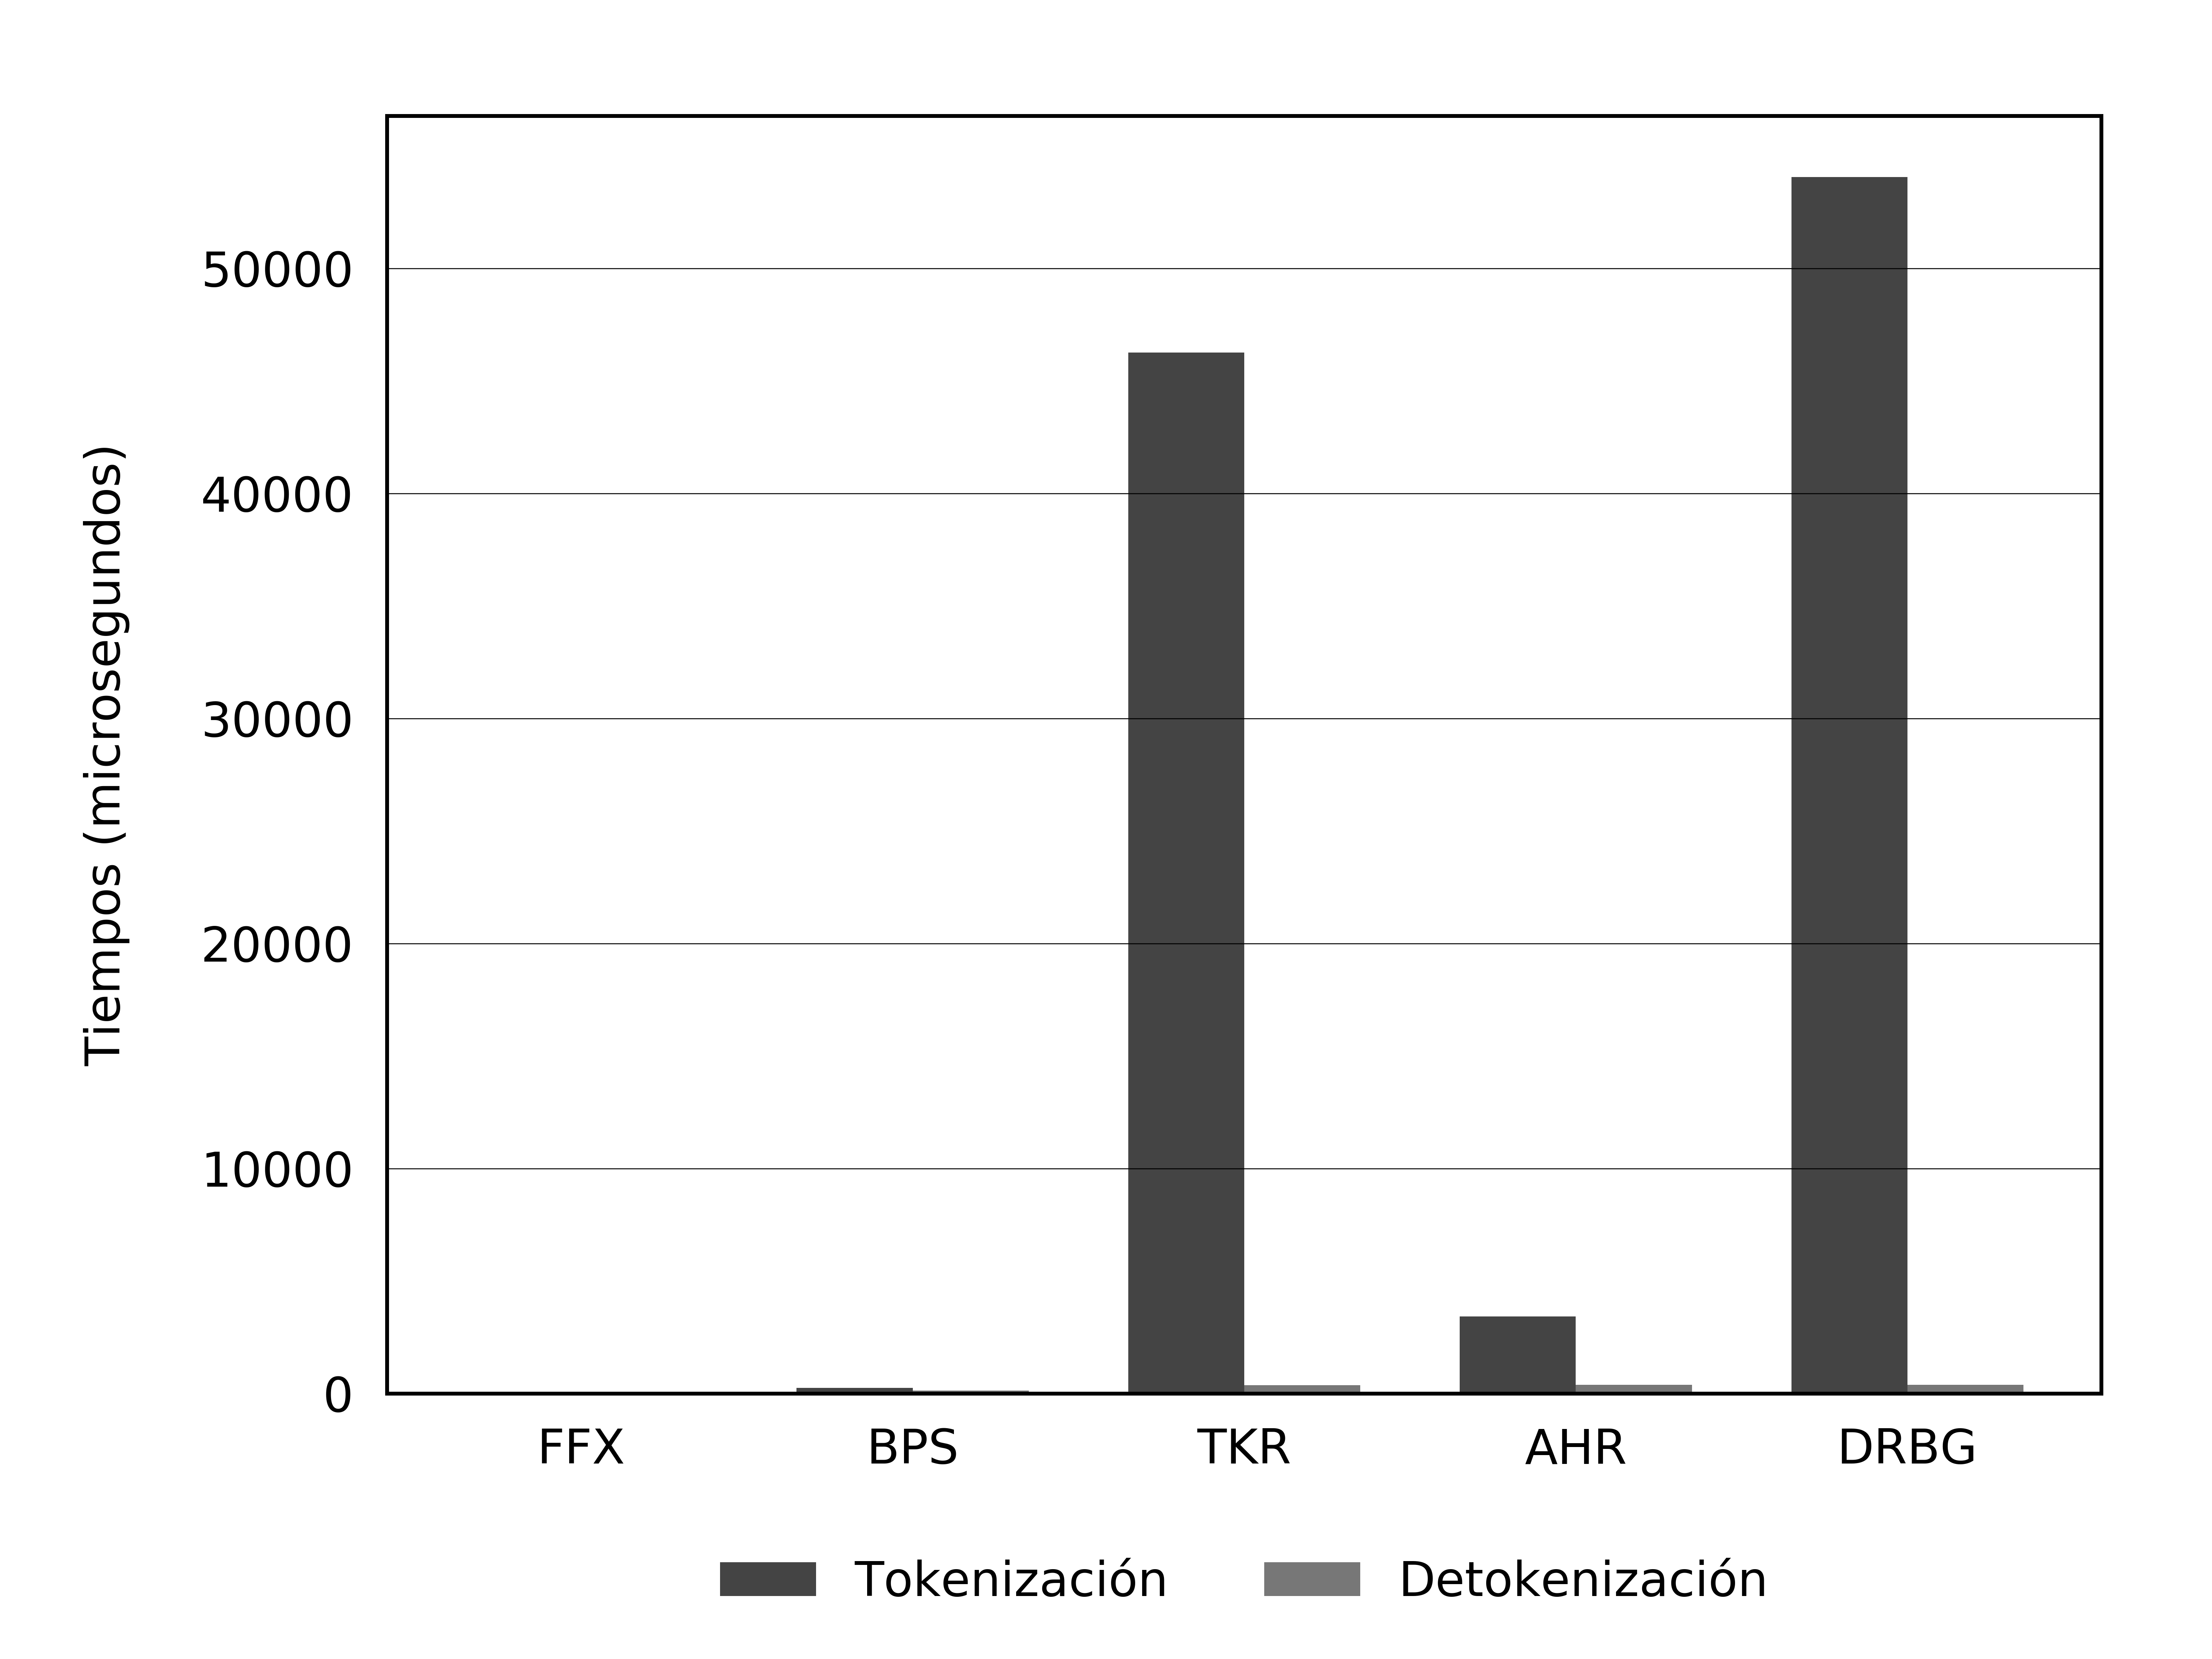
\includegraphics[width=0.9\linewidth]
        {articulo-rci/tiempos_unitarios.png}
        \caption{Tokenización y detokenización.}
    \end{figure}
  \end{frame}

  \begin{frame}{Resultados}
    \begin{figure}[H]
      \centering
      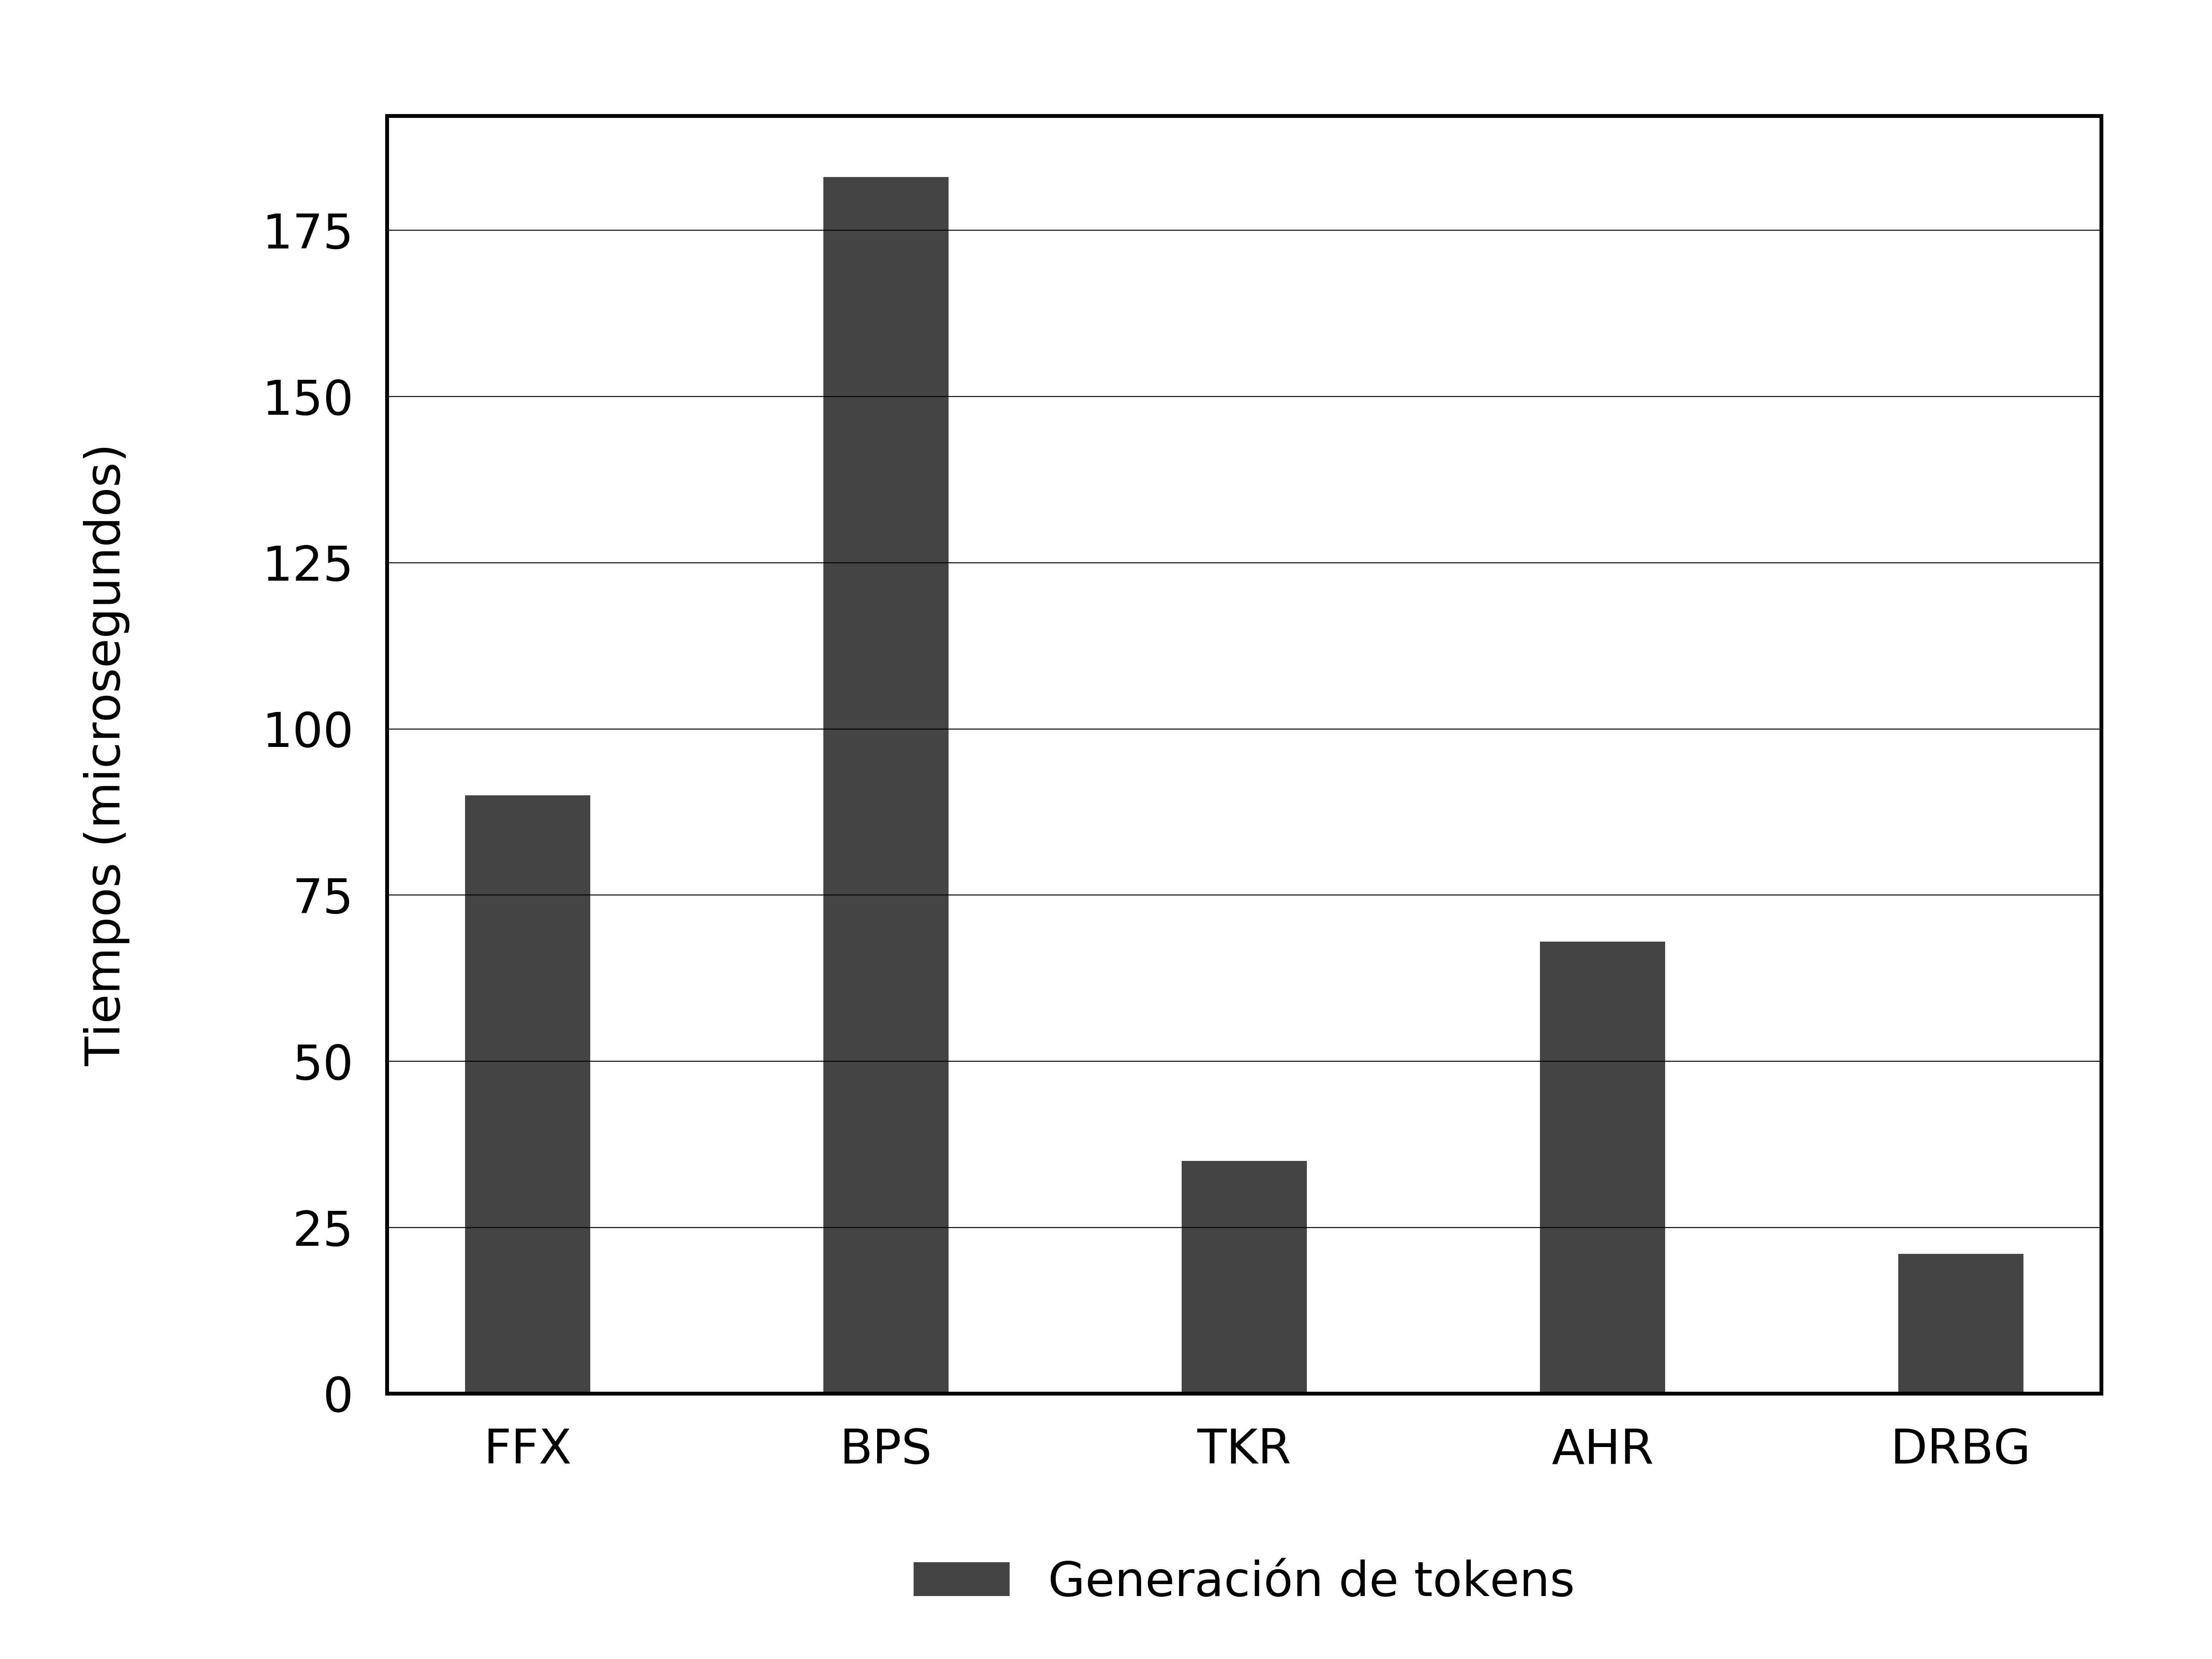
\includegraphics[width=0.9\linewidth]
        {articulo-rci/tiempos_tokenizacion.png}
        \caption{Generación de tokens.}
    \end{figure}
  \end{frame}

  \begin{frame}{Conclusiones}
    \begin{itemize}
      \item La tokenización es una aplicación de la criptografía.
      \item La denominación \textit{no criptográfica} del PCI es contradictoria.
      \item Los algoritmos reversibles son más últiles cuando se necesita tanto
        tokenizar como detokenizar con frecuencia.
      \item Los algoritmos irreversibles son más últiles cuando se requiere
        detokenizar con frecuencia.
    \end{itemize}
  \end{frame}

  \begin{frame}[allowframebreaks]{Bibliografía}
    \printbibliography
  \end{frame}

  \begin{frame}{}
    \centering \Huge
    \textsc{Gracias por su atención.}
  \end{frame}

  % Espacio entre párrafos
  \setlength{\parskip}{0.0em}

  {\setbeamertemplate{footline}{}
  \frame{\titlepage}}

\end{document}
